\documentclass{article}

% Language setting
% Replace `english' with e.g. `spanish' to change the document language
\usepackage[english]{babel}

% Set page size and margins
% Replace `letterpaper' with`a4paper' for UK/EU standard size
\usepackage[letterpaper,top=2cm,bottom=2cm,left=3cm,right=3cm,marginparwidth=1.75cm]{geometry}

% Useful packages
\usepackage{amsmath}
\usepackage{graphicx}
\usepackage[colorlinks=true, allcolors=blue]{hyperref}
\usepackage[section]{placeins}
\graphicspath{
    {../plots}
}

\title{Randomized Search}
\author{Josh Gillette}
\date{March 6, 2024}

\begin{document}
\maketitle

\section{Introduction}
Four random search algorithms: randomized hill climbing, simulated annealing, a genetic algorithm, and MIMIC were implemented in conjunction with three optimization problems: Knapsack, Flip Flop, and Four Peaks. Each of these optimization problems are leveraged to highlight the strengths of a randomized search algorithm. This is conveyed by running each search algorithm on three different problem sizes for every optimization problem. Further, each search algorithm instance was manually and specifically tuned for both the respective optimization problem and problem size.

Additionally, a subset of these search algorithms were then used to determine a neural network's weights. Utilizing a past, large-featured data set several neural networks were again manually tuned and then compared to a neural network that relies on back propagation to determine weight values.

\section{Optimization}

\subsection{The Problems}

As mentioned above, each optimization problem was run on three problem sizes referred to as small (size 10), medium (size 30), and large (size 50). Additionally every optimization problem ran on a given randomized search algorithm was repeated five times with differing random seeds. The resulting values were then aggregated across the five trials. Lastly, Four Peaks used a t\_pct=0.15 and Knapsack used pre-randomized weights and values.
\subsubsection{Knapsack}
Knapsack is a pragmatic and intuitive optimization problem that asks, given a set of items with a defined value and weight, what subset of those items maximize the cumulative value while the cumulative weight does not exceed the knapsack's weight limit. For larger problem sizes where greatly differing combinations may end up being optimal, it can be seen how this problem would benefit from a population of solutions that iterate on one another towards a better solution. These varying potential solution sets all lend this problem to more opportunities in parallelization.

For each problem size a knapsack was created with unique values from 1 to $size$ and random weights between 1 and 20 (inclusive).

\subsubsection{Flip Flop}
Flip Flop is a simple optimization problem where the number of alternating bits in a bit string maximize a fitness function. Flip Flop represents a more straight forward optimization problem without traps that may add dimension and complexity to the problem. In addition to measuring a search algorithm's fitness, this problem provides an opportunity to compare the efficiency of the  algorithms.

\subsubsection{Four Peaks}
Four Peaks is an intriguing optimization problem whose fitness is evaluated by counting the 0s in the front and 1s in the back of a bit string and then taking the maximum of the two counts. It is designed to catch certain random search algorithms by containing two local optima/peaks; additionally if the maximum value is larger than a percent threshold a bonus is added. A search algorithm that yields a high fitness value would need the ability to model the structure of the two peaks in such a way that also achieves the bonus.

\subsection{Results}

\subsubsection{Genetic Algorithm}

With respect to Knapsack, a genetic algorithm performed best in several areas. First, it proved to be the overall fittest algorithm, especially in the large problem size by a margin of $\sim15\%$. Further, the genetic algorithm performed well on wall clock time, beating randomized hill climbing and MIMIC by a sizeable gap and only being bested by simulated annealing. Lastly, the genetic algorithm's standard deviation was tight across all trials. This provides the secondary benefit of increased reliability for the genetic algorithm in settings where multiple trials may not be possible. Lastly, the genetic algorithm has the desirable benefit of its fitness score not being correlated to iterations, which tracks with the linear wall clock time observed.

\begin{center}
    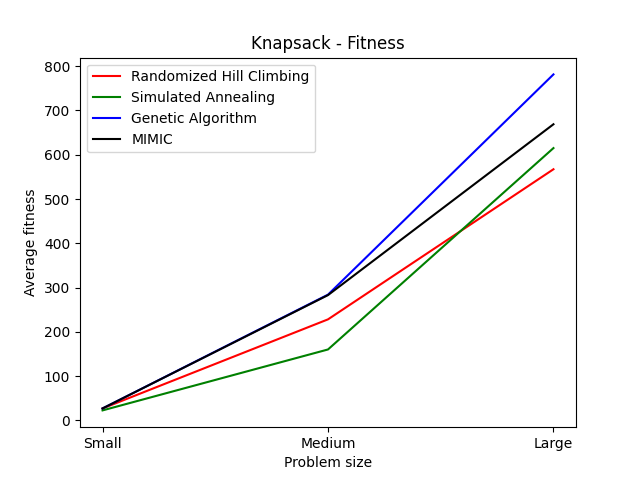
\includegraphics[width=.49\linewidth]{knapsack_fitness.png}
    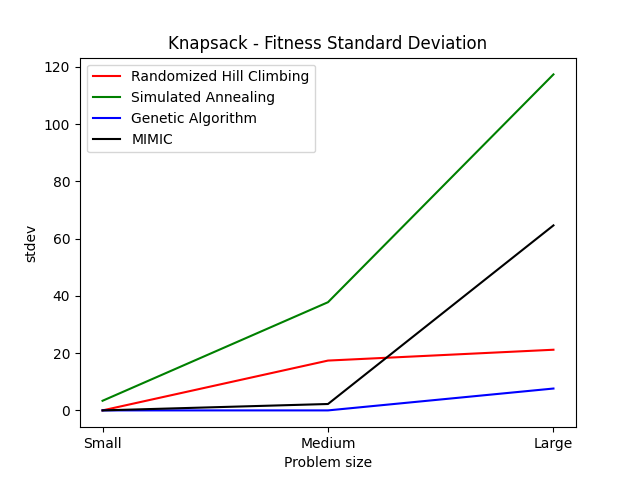
\includegraphics[width=.49\linewidth]{knapsack_stdev.png}
\end{center}

\begin{center}
    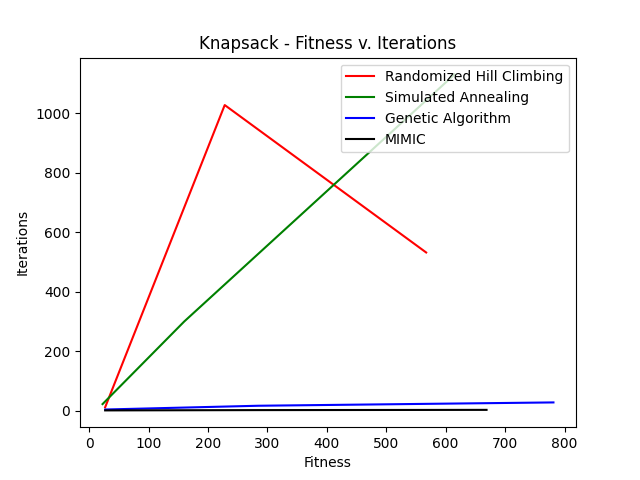
\includegraphics[width=.49\linewidth]{knapsack_fitness_iters.png}
    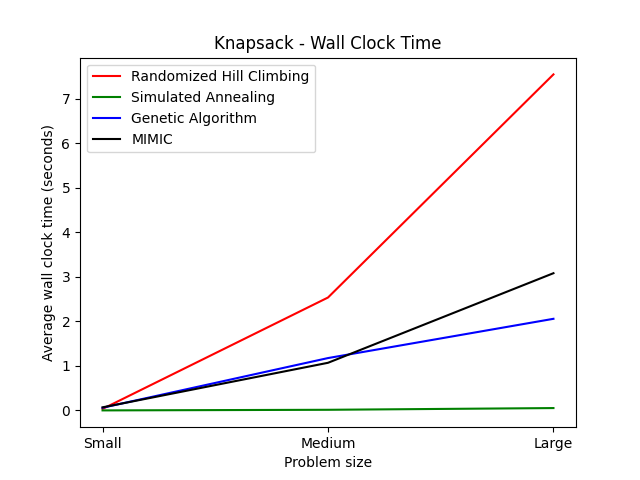
\includegraphics[width=.49\linewidth]{knapsack_time.png}
\end{center}

As alluded to, a genetic algorithm lends itself well to a problem similar to Knapsack. The genetic algorithm continually recreates its population by passing through, mutating, or crossing over members of the previous population. Knapsack has a wide range of potential solutions that can be handled by the population size, and minor mutations or changes will slowly work toward a value convergence for the Knapsack.

This is reflected in the tuning of the hyperparameters for this problem. The tuning often followed high population sizes (200, 900, 950) (this is shorthand hand for the hyperparameters corresponding to (small, medium, large) problem sizes), low but increasing max\_iterations (4, 18, 35), as well as a lower but also increasing mutation probability (0.001, 0.005, 0.02). The low mutation probability being advantageous may be a product of the specific Knapsack value and weight input.

\subsubsection{Simulated Annealing}

Observing Flip Flop, simulated annealing performed well in fitness (its plot is overlapped with MIMIC) as did all other algorithms. However, it sets itself apart in efficiency. Simulated annealing's wall clock times are significantly better the other algorithms and this improvement scales well with problem size. Simulated annealing also performs well consistently as it showcases a low standard deviation (again overlapped with MIMIC) between trials. There is a direct and non-linear correlation between simulated annealing's fitness and iterations, but the nature of the algorithm's quick iterations justified the tuning of a higher max\_iters.

\begin{center}
    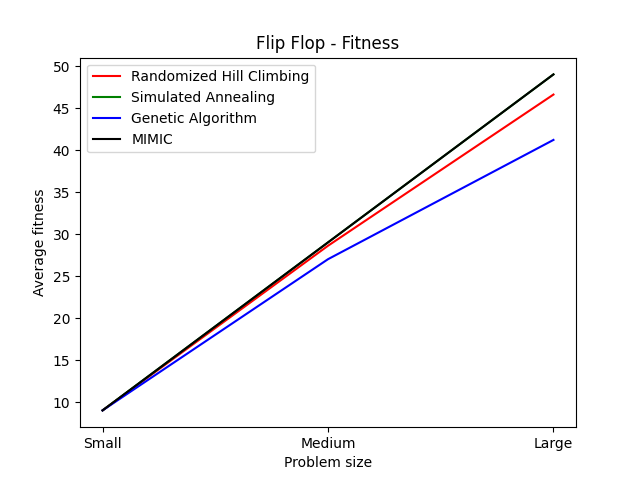
\includegraphics[width=.49\linewidth]{flip_flop_fitness.png}
    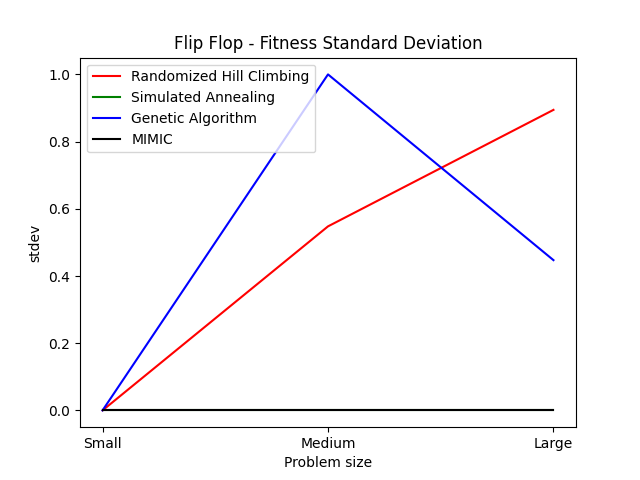
\includegraphics[width=.49\linewidth]{flip_flop_stdev.png}
\end{center}

\begin{center}
    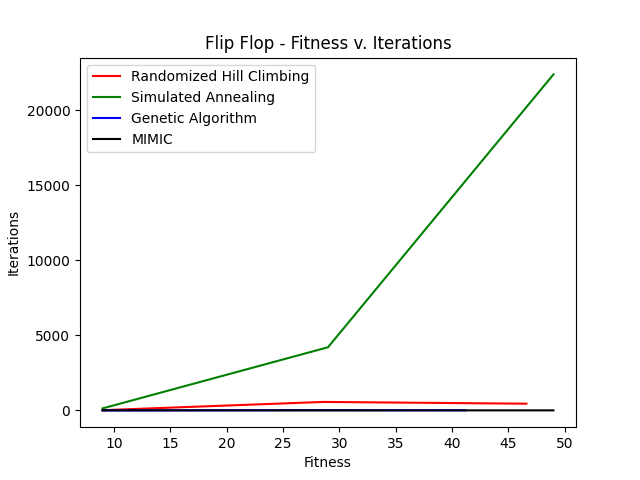
\includegraphics[width=.49\linewidth]{flip_flop_fitness_iters.png}
    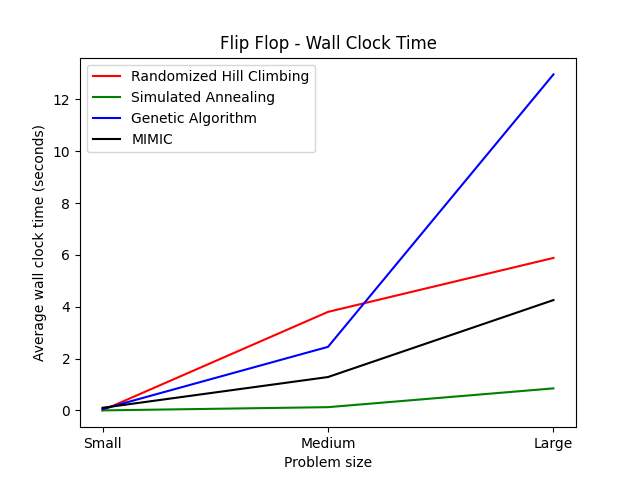
\includegraphics[width=.49\linewidth]{flip_flop_time.png}
\end{center}

Flip Flop lends itself well to simulated annealing as the algorithm's able to perform its discovery of candidate solutions and cool off in a uniform problem arena. The hyperparameter tuning used a standard geometric decay, but found max\_attempts (14, 90, 200) and max\_iters (230, 8,000, 70,000) tuning to be beneficial in maximizing fitness while not sacrificing wall clock time.

\subsubsection{MIMIC}

MIMIC performs markedly better than the others algorithms on the Four Peaks problem at large problem sizes. It also yields a low standard deviation between runs. This improvement does come at a cost in wall clock time, but can be justified due to its better performance. MIMIC also shows the benefit of its fitness not being correlated to its iterations.

\begin{center}
    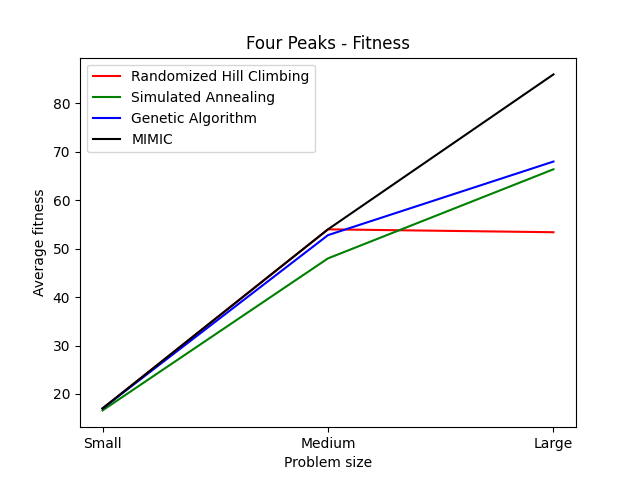
\includegraphics[width=.49\linewidth]{four_peaks_fitness.png}
    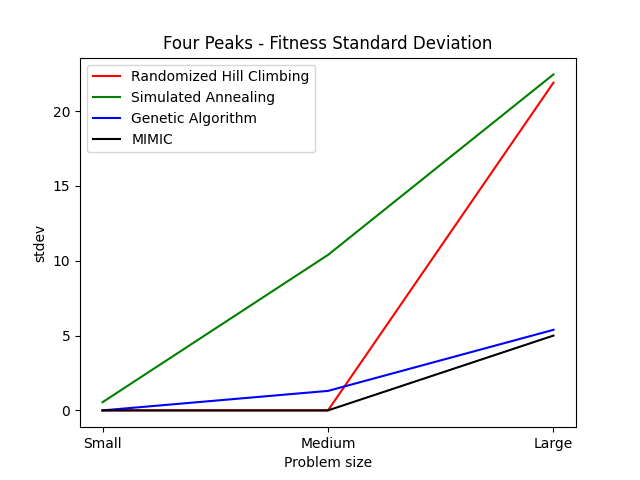
\includegraphics[width=.49\linewidth]{four_peaks_stdev.png}
\end{center}

\begin{center}
    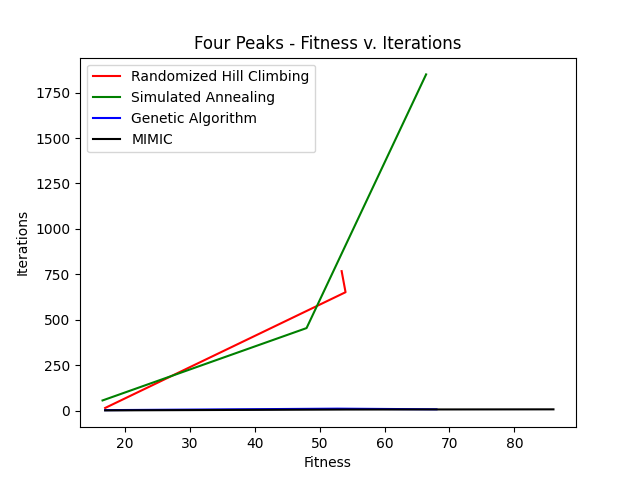
\includegraphics[width=.49\linewidth]{four_peaks_fitness_iters.png}
    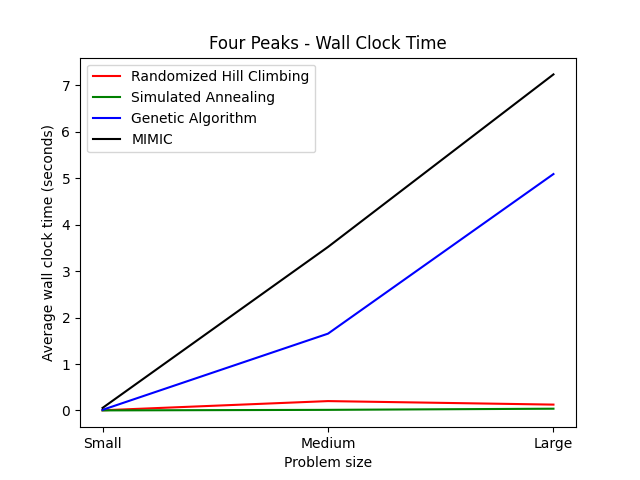
\includegraphics[width=.49\linewidth]{four_peaks_time.png}
\end{center}

The behavior of MIMIC in Four Peaks aligns with the algorithms characteristics. MIMIC's sampling of regions of the input space that are most likely to contain the minimum cost and effective density estimator are intensive processes for large problem sizes. Fortunately, as shown above this scales linearly for wall clock time.

MIMIC's hyperparameters often followed low values max\_attempts (1, 3, 1) and max\_iters (1, 6, 8), which follows from the above plots conveying MIMIC's iteration count not being correlated to its fitness improvements. MIMIC's population sizes non-linearly vary across problem sizes (500, 20000, 2000) which can maybe be explained to understanding the global structure of the optimization landscape requiring an acceptable population size.

\subsection{Overall Analysis}

From above visuals articulate the relationship between fitness, fitness standard deviation, wall clock time, iterations, and problem size have with one another. There are several relationships that arise from these.

One of which being the lack of a strong relationship between iterations and wall clock time. In Flip Flop, simulated annealing has the overall smallest wall clock time, but requires the most amount of iterations to improve fitness. Yet in Four Peaks MIMIC has the largest wall clock time, but it's fitness gains have no relationship to iterations. From this it becomes clear a simulated annealing iteration is considerably quicker than a MIMIC iteration.

Another is the approximate proclivity for the various algorithm's fitness values to converge or behave similarly. Between the nine points of comparison for fitness, the algorithms converge to similar fitness values at about seven points; with only really one point (Four Peaks, large) showing greatly different fitness values. It can be taken from this that an algorithms efficiency may often be a better indicator of usefulness in the real world.

There are multiple interesting way to further experiment with these search algorithms and optimization problems. The first of which would definitely be larger problem sizes. Testing with only three problem sizes that are just 1.5-3x larger than one another does not provide great coverage for these algorithms. This was a limitation on personal processing power and time, but to fully understand these algorithms and problems require expanded problem sizes.

While manually tuning these algorithms, the convergence point for each algorithm/problem combination was found and then the hyperparameters were further modified to lend towards efficiency while still maintaining the convergence point. It would be interesting to approach the tuning from a different direction. Rather that be computationally or modifying the manual approach taken.

Lastly, beyond just increasing the size of the problems, it would be interesting to modify the optimization problems input values manually. For instance, Knapsack's input weights and values or Four Peaks t\_pct value. Whether a set of random values were fed into these problems or strategized solutions, it would be necessary to fully understand these search algorithms.

\section{Neural Networks}

A neural network's weights are values assigned to the connections between neural nodes and represent the relationship one node has with another. These weights play a vital role in the behavior of a neural network, and will be determined by one of two ways: back propagation or by use of a random search algorithm. A credit dataset that was previously fit to a neural network that utilizes back propagation will be compared to three other neural networks that instead uses randomized search algorithms (randomized hill climbing, simulated annealing, and a genetic algorithm). The credit dataset contains 23 features and 30,000 rows that the neural network will train on.

Just as previously, each search algorithm was manually tuned with the same method as the previous section. Hyperparameters were matched between the two types of neural networks which include matching activation function (relu), solvers (lbfgs), and alpha/learning rate (0.00001).

\begin{center}
    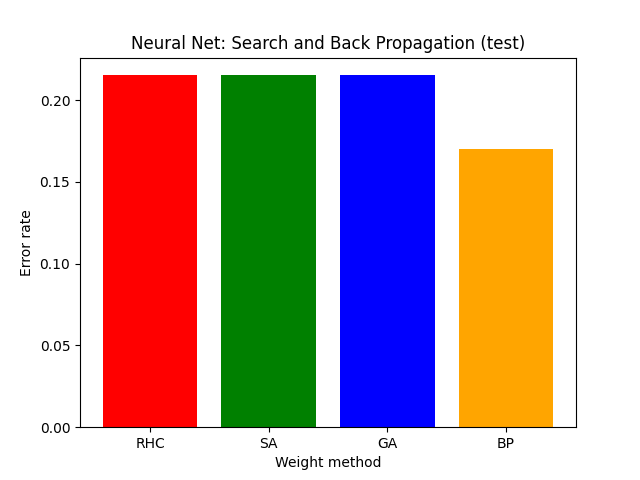
\includegraphics[width=.49\linewidth]{neural_test.png}
    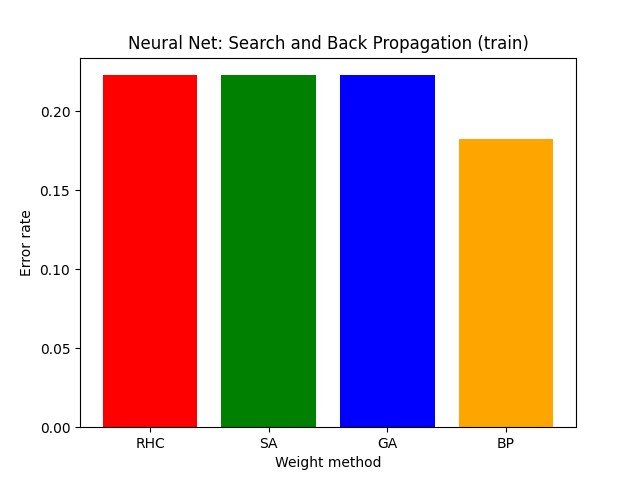
\includegraphics[width=.49\linewidth]{neural_train.png}
\end{center}

\begin{center}
    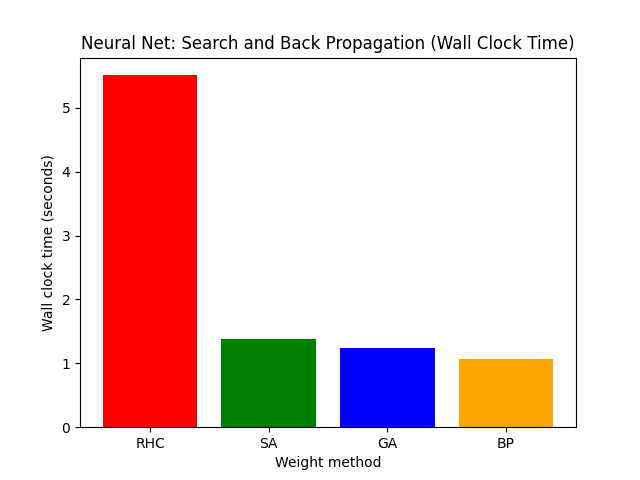
\includegraphics[width=.49\linewidth]{neural_time.png}
    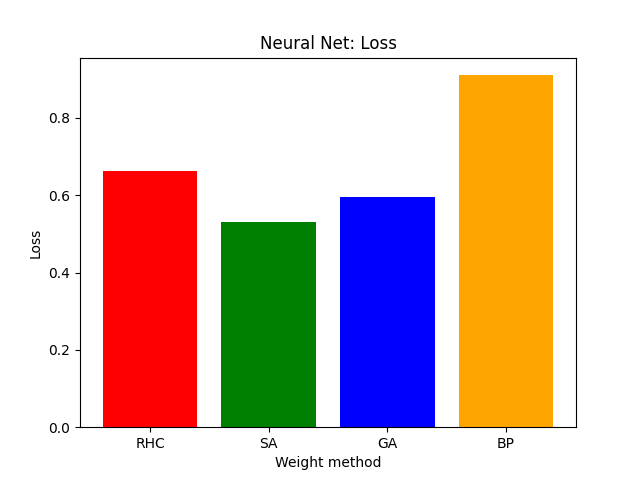
\includegraphics[width=.49\linewidth]{neural_loss.png}
\end{center}

The above plots compare the three randomized search algorithm neural networks (RHC, SA, GA) to the back propagation neural networks (BP). Looking at the top two plots outlining test and train fitting respectively, the three search algorithm neural networks not only yield a higher error rate, but also converge to the same error rate. Wall clock time is considerably worse for randomized hill climbing, and simulated annealing produces a slightly higher time compared to the genetic algorithm and back propagation. Judging by these first three graphs, it appears that the back propagation neural network wholistically performs better than the randomized search algorithm neural networks.

However, the most interesting plot shows the neural networks loss values. Here, lower is better as the loss value conveys the errors made for each instance in the validation and training sets. Despite the random search algorithms yielding and converging to higher error rates, the loss value of each randomized search algorithm backed neural network performs better than the back propagation neural network.

The loss values are more indicative of the quality of the neural network's weights, while the error rates represent the applied value of the model. Concluding which neural network method is better depends on the metrics that are valued. If minimizing error rate is the entire goal, then a back propagated neural network may be the best move. Should precise predictions rather be the model's primary goal, than a randomized search algorithm driven neural network may be desirable.

\end{document}
